\documentclass[aspectratio=43,t]{beamer}

% Colors
\usepackage{color}
\definecolor{mainorange}{HTML}{EC811B}
\definecolor{lightgrey}{HTML}{888888}
\definecolor{librepcb}{RGB}{41,214,130}

% Syntax highlighting
\usepackage{minted}
\usepackage{alltt}
\newcommand\hi[1]{{\color{mainorange} \textbf{#1}}}

% Directory trees
\usepackage{dirtree}

% Tikz
\usepackage{tikz}
\usepackage{tikzsymbols}
\usetikzlibrary{calc}
\usetikzlibrary{positioning}
\usetikzlibrary{fit}
\usetikzlibrary{matrix}
\usetikzlibrary{shapes, shapes.callouts}
\usetikzlibrary{shadows}
\usetikzlibrary{arrows, arrows.meta}
\usetikzlibrary{backgrounds}
\pgfdeclarelayer{background}
\pgfdeclarelayer{foreground}
\pgfsetlayers{background,main,foreground}
\tikzstyle{lpbox}=[rectangle, draw=black, rounded corners, fill=librepcb, drop shadow,
                   text centered, anchor=north, text=white]
\tikzstyle{lpline}=[]
\tikzstyle{lparrow}=[lpline, -{Stealth}]
\tikzstyle{lparrow2}=[lpline, {Stealth}-{Stealth}]

% Various packages
\usepackage{multirow}
\usepackage{array}
\usepackage[framemethod=TikZ]{mdframed}
\usepackage{fontawesome}

% Theme
\usetheme[%
  sectionpage=none,
  subsectionpage=none,
  numbering=fraction,
  progressbar=foot,
]{metropolis}

% Customization
\setbeamertemplate{section in toc}[sections numbered]
\setbeamerfont{title}{size=\fontsize{30}{30}}
\setbeamerfont{block title}{size=\large}
\newcommand\sep{\textcolor{lightgrey}{\rule{\linewidth}{0.05mm}}}

% Meta
\title{LibrePCB}
\subtitle{A new, powerful and intuitive EDA tool for everyone}
\date{\today}
\author{Urban Bruhin}
\institute{}

\begin{document}

% ----------------------------------------------------------------- %

\maketitle

% ----------------------------------------------------------------- %

%\begin{frame}[plain,noframenumbering]
%	\frametitle{Table of Contents}
%	\setcounter{tocdepth}{1}
%	\tableofcontents
%\end{frame}

% ----------------------------------------------------------------- %

\section{About LibrePCB}

\begin{frame}{\secname}
  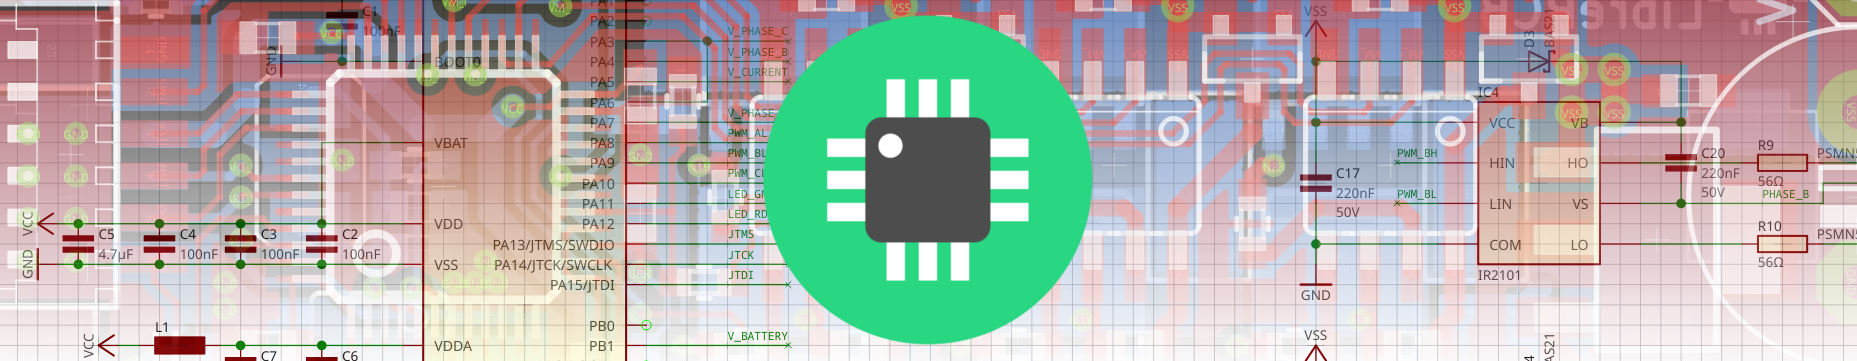
\includegraphics[width=\linewidth]{images/about_header.png} \linebreak\linebreak
  \textbf{Free/OpenSource EDA Suite}
  \begin{itemize}
    \item Multiplatform \faLinux\ \faApple\ \faWindows\
    \item Written from scratch in C++11/Qt5
    \item Development started in February 2013
    \item Website: \url{http://librepcb.org/}
    \item GitHub: \url{https://github.com/LibrePCB/LibrePCB}
  \end{itemize}
\end{frame}
\section{File Format Extensibility}

\begin{frame}{\secname}
  \textbf{Problem}
  \begin{itemize}
    \item File format of other tools were not designed for extensibility
  \end{itemize}
  
  \pause
  
  \textbf{Result}
  \begin{itemize}
    \item Missing or broken support for 3D models
    \item Missing or broken support for SPICE models
    \item Not ready for future extensions
  \end{itemize}
\end{frame}

\begin{frame}{\secname}
  \textbf{Solution}
  \begin{itemize}
    \item 1 entity = 1 directory
  \end{itemize}
  
  \pause
  
  \begin{center}
    \color{blue}
    \vspace*{-\baselineskip}\leavevmode % reduce space
    \begin{tikzpicture}[node distance=5mm, hint/.style={rectangle callout, fill=librepcb!30, text=black, rounded corners}]
      % uuid
      \node (dir) [] {
        \large\faFolderOpenO
      };
      \node (uuid) [anchor=west] at (dir.east) {
        \large\texttt{2d9ba47b-3ff1-44db-aa4e-0bfec1f12ea8}
      };
      \node [hint, above right=of uuid, anchor=south east, callout absolute pointer=(uuid.north)] {
        Directory name = entity UUID
      };
      
      % version file
      \node (file1) [anchor=north west] at (dir.south east) {
        \large\faFileTextO\ \large\texttt{.librepcb-pkg}
      };
      \draw (dir.south) |- (file1.west);
      \node [hint, below right=5mm and 2cm of file1.north east, anchor=north west, callout absolute pointer=(file1.east), text width=4.5cm] {
        Plain text file\\
        $\bullet$ Forward compatible\\
        $\bullet$ Filename = entity type\\
        $\bullet$ Content = format version 
      };
      
      % entity file
      \node (file2) [anchor=north west] at (file1.south west) {
        \large\faFileTextO\ \large\texttt{package.lp}
      };
      \draw (dir.south) |- (file2.west);
      \node [hint, below right=17mm and 8mm of file2, anchor=north west, callout absolute pointer=(file2.east), text width=4.5cm] {
        S-Expression file containing the actual entity data
      };
      
      % 3dmodel
      \onslide<3->{
        \node (file3) [anchor=north west] at (file2.south west) {
        \large\faFileImageO\ \large\texttt{3dmodel.wrl}};
        \draw (dir.south) |- (file3.west);
      }
      
      % step model
      \onslide<4->{
        \node (file4) [anchor=north west] at (file3.south west) {
        \large\faFileImageO\ \large\texttt{3dmodel.step}};
        \draw (dir.south) |- (file4.west);
      }
      
      % spice model
      \onslide<5->{
        \node (file5) [anchor=north west] at (file4.south west) {
        \large\faFileTextO\ \large\texttt{spice.mod}};
        \draw (dir.south) |- (file5.west);
      }
    \end{tikzpicture}
  \end{center}
\end{frame}
\section{Self-Contained Projects}

\begin{frame}{\secname}
  \textbf{Problem}
  \begin{itemize}
    \item Projects depend on information stored outside the project
    \begin{itemize}
      \item Library entities, settings, fonts, ...
    \end{itemize}
  \end{itemize}
  
  \pause
  
  \textbf{Result}
  \begin{itemize}
    \item Projects are not portable (e.g. \textit{"Library not found"} errors)
    \item Generated production data is not reproducible
    \item Source code is harder to maintain (more changes are breaking)
  \end{itemize}
  
  \pause
  
  \textbf{Solution}
  \begin{itemize}
    \item Embed as much information as possible into projects
    \begin{itemize}
      \item Library entities (forced, not optional)
      \item All relevant settings
      \item Fonts \textit{(work in progress...)}
    \end{itemize}
  \end{itemize}
\end{frame}
\section{Version Control Systems}

\begin{frame}{\secname}

  \begin{columns}[onlytextwidth]
    \begin{column}{\textwidth-3.5cm}
      \textbf{Problem}
      \begin{itemize}
        \item Important and unimportant data mixed
        \item Unclear which files to version control
      \end{itemize}

      \pause

      \textbf{Result}
      \begin{itemize}
        \item Local changes even if nothing modified
        \item Very large and opaque diffs/commits
        \item Important files accidentally ignored
      \end{itemize}

      \pause

      \textbf{Solution}
      \begin{itemize}
        \item Many small files for higher granularity
        \item Unimportant data strictly separated
        \item Automatic creation of \texttt{.gitignore}
      \end{itemize}
    \end{column}

    \hfill

    \begin{column}{3.5cm}
      \color{blue}\dirtree{%
        .1 MyProject.
        .2 .gitignore.
        .2 boards.
          .3 default.lp.
        .2 core.
          .3 circuit.lp.
          .3 erc.lp.
          .3 settings.lp.
%        .2 library.
%          .3 \dots.
        .2 output.
          .3 \dots.
        .2 schematics.
          .3 power.lp.
          .3 logic.lp.
        .2 user.
          .3 \dots.
      }
    \end{column}
  \end{columns}
\end{frame}

\section{Version Control Systems}

\begin{frame}[fragile]{\secname}
  \begin{minted}[baselinestretch=.8,style=trac]{diff}
--- a/test.kicad_pcb
+++ b/test.kicad_pcb
@@ -3,7 +3,7 @@
   (general
     (no_connects 0)
-    (area 41.834999 87.554999 233.755001 153.745001)
+    (area 20.171999 28.969758 233.755001 157.374234)
     (drawings 4)
@@ -21,7 +21,7 @@
     (36 B.SilkS user)
-    (37 F.SilkS user)
+    (37 F.SilkS user hide)
     (38 B.Mask user hide)
@@ -62,7 +62,7 @@
     (aux_axis_origin 0 0)
-    (visible_elements FFFC4601)
+    (visible_elements FFFC4609)
     (pcbplotparams
       (layerselection 0x00030_80000001)\end{minted}
  
  \scriptsize{
    KiCad 4.0.2+dfsg1-stable:
    zoom around,
    hide "F.SilkS",
    show "Through Via"
  }
\end{frame}

\begin{frame}[noframenumbering]{\secname}
  \textbf{Problem}
  \begin{itemize}
    \item Files are \textbf{not really} human readable
  \end{itemize}

  \pause

  \textbf{Result}
  \begin{itemize}
    \item Diffs are very hard to understand
    \item Limited use of version control systems
  \end{itemize}

  \pause

  \textbf{Solution}
  \begin{itemize}
    \item Don't just consider text-based file formats as human readable!
    \item Control every tiny detail of the generated files
    \item Consider opaque parts of files as bugs and fix them
  \end{itemize}
\end{frame}

\section{Library Management}

\begin{frame}{\secname}
  \textbf{Problem}
  \begin{itemize}
    \item Tools do not (completely) handle library management
    \begin{itemize}
      \item No integrated library browser to discover and install libraries
      \item Symbols and footprint splitted up in separate libraries
      \item No dependency management
    \end{itemize}
  \end{itemize}
  
  \pause
  
  \textbf{Result}
  \begin{itemize}
    \item It's up to the user to manage his libraries (which is a pain)
  \end{itemize}
\end{frame}

\begin{frame}[noframenumbering]{\secname}
  \begin{center}
    \vspace*{-2\baselineskip}\leavevmode % reduce space
    \begin{tikzpicture}
      \onslide<1->{\node (img1) [anchor=north west] at (0cm,0cm) {
        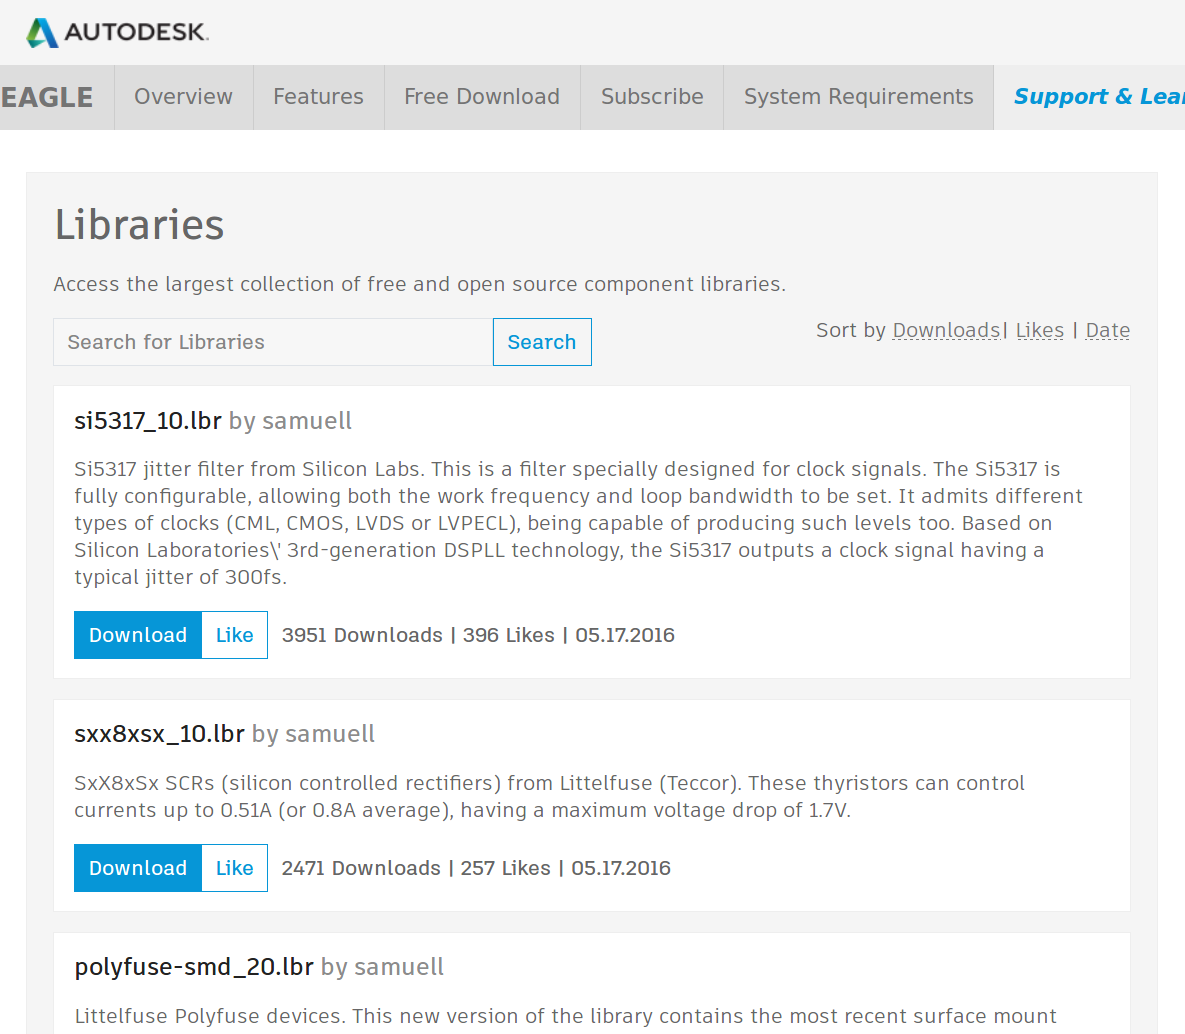
\includegraphics[height=.85\textheight]{images/eagle_libraries_website.png}
      };}
      \onslide<2->{\node (img2) [anchor=north west] at (2cm,-1cm) {
        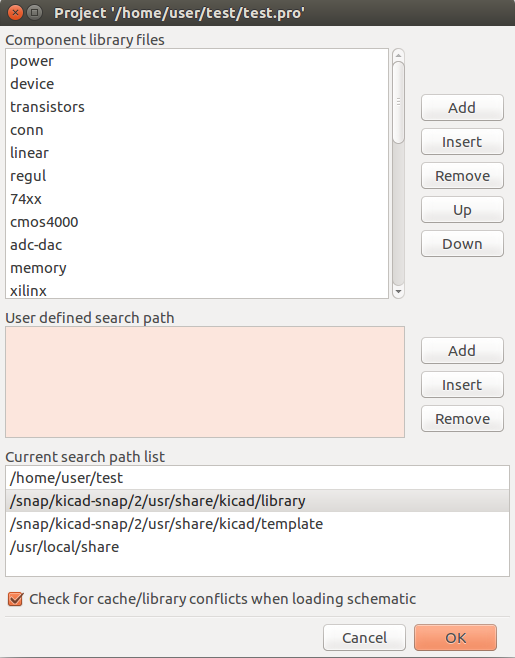
\includegraphics[height=.85\textheight]{images/kicad_component_libraries.png}
      };}
      \onslide<3->{\node (img3) [anchor=north west] at (4cm,-2cm) {
        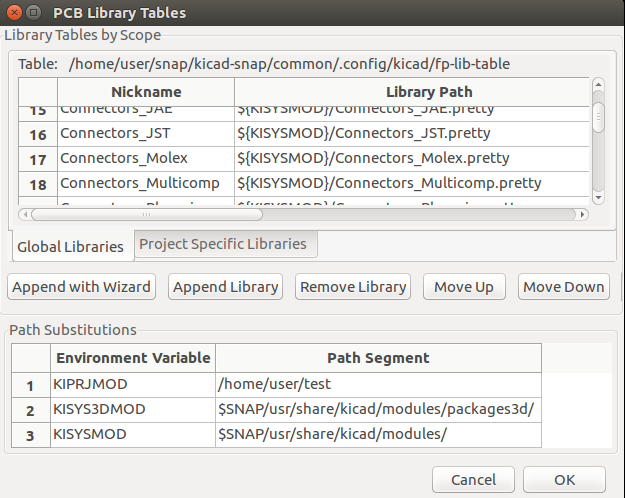
\includegraphics[height=.65\textheight]{images/kicad_library_tables.png}
      };}
      \onslide<4->{\draw (img2.center) node[scale=12] {
        \color{red}{\faQuestion}
      };}
    \end{tikzpicture}
  \end{center}
\end{frame}

\begin{frame}[noframenumbering]{\secname}
  \textbf{Solution}
  \begin{itemize}
    \item Integrated library manager with dependency management
    \item Libraries can contain any entity type (symbols, footprint, ...)
    \item The application handles basically \textbf{everything} for you
  \end{itemize}

  \begin{center}
    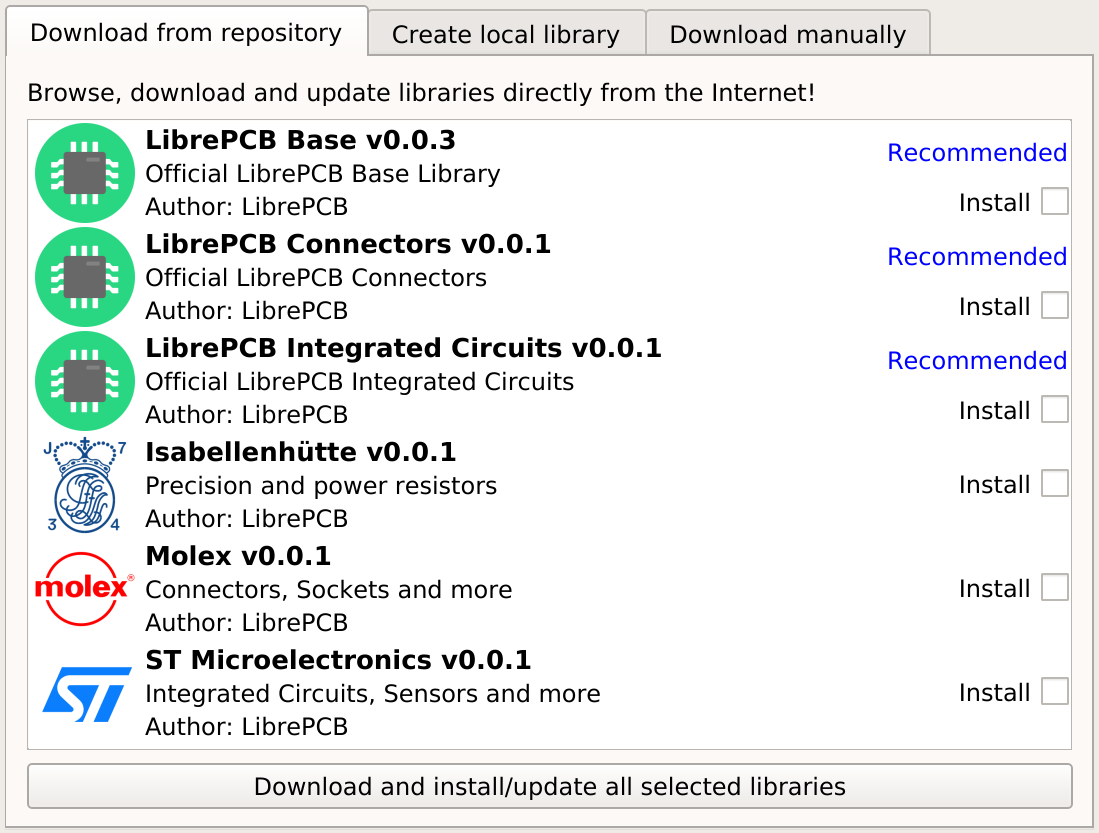
\includegraphics[height=5cm]{images/library_manager.png}
  \end{center}
\end{frame}
\section{Quality of Libraries}

\begin{frame}{\secname}
  \textbf{Problem}
  \begin{itemize}
    \item Quality of available libraries is very bad
  \end{itemize}

  \pause

  \textbf{Solution}
  \begin{itemize}
    \item \textit{"You need to create your own libraries to fit your needs."}
  \end{itemize}

  \pause

  \begin{tikzpicture}[remember picture,overlay]
    \draw (current page.center) node[rotate=35,scale=9] {
      \color{red}\textbf{NO!}
    };
    %\pause
    %\draw (current page.south) ++ (0,.15\paperheight) node[scale=2] {
    %  \color{red}\textbf{Why is the quality of libraries that bad?}
    %};
  \end{tikzpicture}
\end{frame}

\section{Library References}

\begin{frame}{\secname}
  \textbf{Problem}
  \begin{itemize}
    \item Everything is referenced by name
    \item References only work within the same library
  \end{itemize}

  \pause

  \textbf{Result}
  \begin{itemize}
    \item Broken references after changing names
    \item Name conflicts because they are not unique
    \item Many duplicates accross different libraries
  \end{itemize}

  \pause

  \textbf{Solution}
  \begin{itemize}
    \item Every entity is identified by a random UUID
    \item References always by UUID, never by name
    \item Entities can be referenced accross different libraries
  \end{itemize}
\end{frame}

\begin{frame}[fragile]{\secname}
  \begin{minted}[baselinestretch=.9,escapeinside=||]{scm}
(librepcb_symbol
 (uuid |\colorbox{yellow}{f0061936-5169-49c9-bfa5-4efc8108cd1c}|)
 (name "Connector 1x4")
 ...
 (pin |\colorbox{yellow}{169d6728-7108-4600-aa48-765711db01bc}| (name "1")
  (pos -20.32 40.64) (rot 0.0) (length 5.08)
 )
 (pin |\colorbox{yellow}{1c49822e-fd83-452a-a7a6-f4ae1357a0c7}| (name "2")
  (pos 20.32 -40.64) (rot 180.0) (length 5.08)
 )
 (pin |\colorbox{yellow}{208bd2b9-ed07-4df5-b5ab-a89fb03378d5}| (name "3")
  (pos 20.32 -38.1) (rot 180.0) (length 5.08)
 )
 (pin |\colorbox{yellow}{2684075c-566e-43fb-b025-17cf43badaf4}| (name "4")
  (pos 20.32 -12.7) (rot 180.0) (length 5.08)
 )
)
  \end{minted}
\end{frame}

\section{Library Browser}

\begin{frame}{\secname}
  \textbf{Problem}
  \begin{itemize}
    \item Entities are organized by their containing library
    \item No way to assign categories and/or keywords to library entities
  \end{itemize}

  \pause

  \textbf{Result}
  \begin{itemize}
    \item Users need to carry about (absolutely irrelevant) library names
    \item Entities are very hard to find in the library browser
  \end{itemize}
\end{frame}

\begin{frame}[noframenumbering]{\secname}
  \begin{columns}[c]
    \begin{column}{.6\textwidth}
      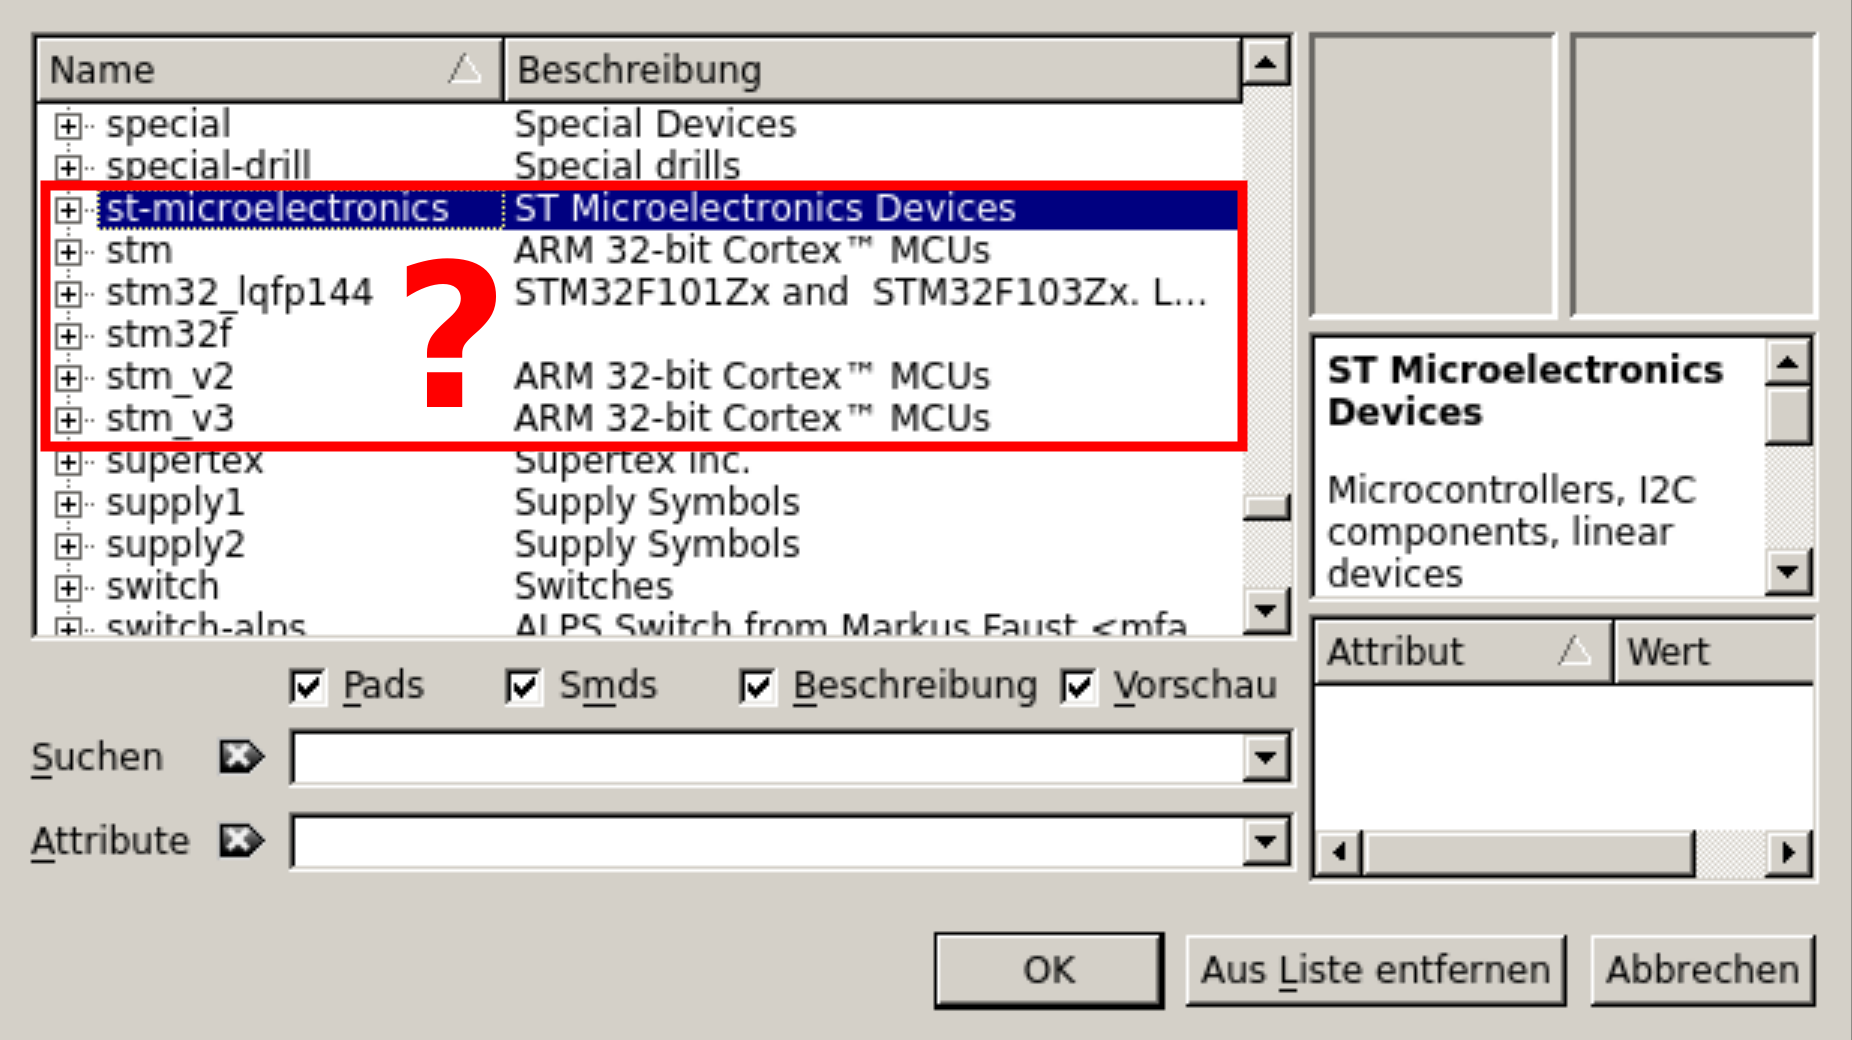
\includegraphics[width=\textwidth]{images/eagle_library_browser.png}
    \end{column}

    \begin{column}{.48\textwidth}
      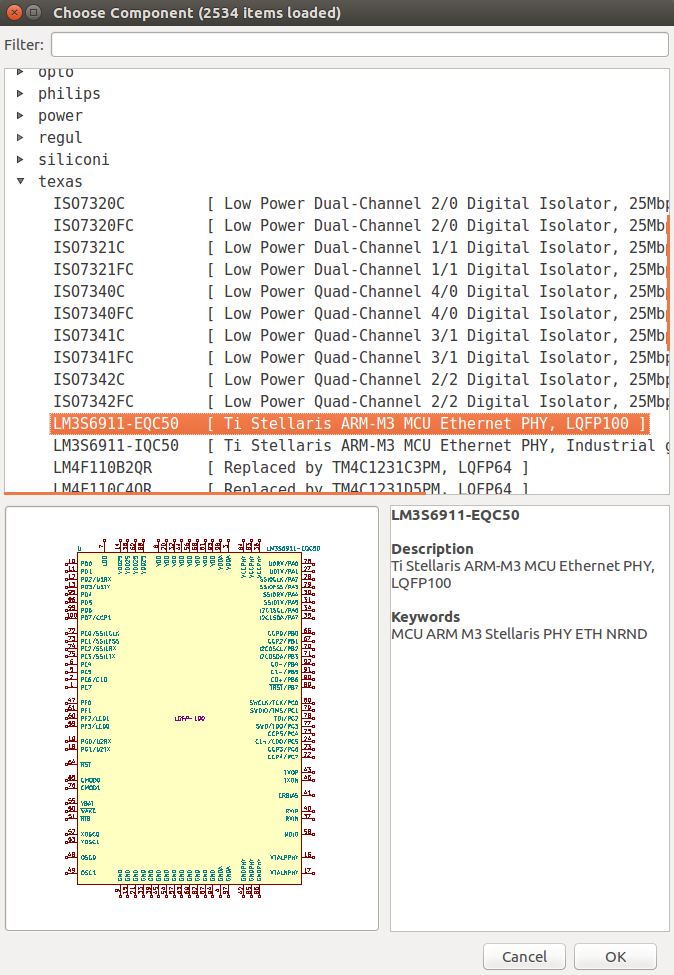
\includegraphics[width=\textwidth]{images/kicad_library_browser.png}
    \end{column}
  \end{columns}
\end{frame}

\begin{frame}{\secname}
  \textbf{Solution}
  \begin{itemize}
    \item Libraries can contain \textbf{categories}
    \item Entities can be assigned to these categories
    \item Entities can have keywords
  \end{itemize}
  \begin{center}
    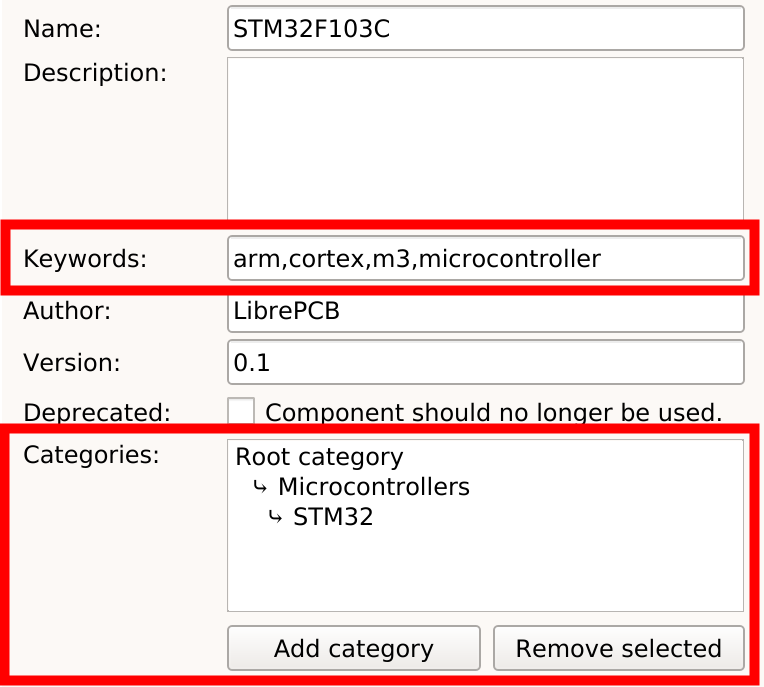
\includegraphics[width=.45\textwidth]{images/library_keywords_and_categories.png}
  \end{center}
\end{frame}

\begin{frame}[noframenumbering]{\secname}
  \begin{center}
    \includegraphics<1>[width=.95\textwidth]{images/library_browser_categories_stm32.png}
    \includegraphics<2>[width=.95\textwidth]{images/library_browser_categories_diode.png}
    \includegraphics<3>[width=.95\textwidth]{images/library_browser_keywords.png}
  \end{center}
\end{frame}

\section{Symbol Variants}

\begin{frame}{\secname}
  \textbf{Problem}
  \begin{itemize}
    \item Impossible to have different symbols for the same component\\
          e.g. Resistor: 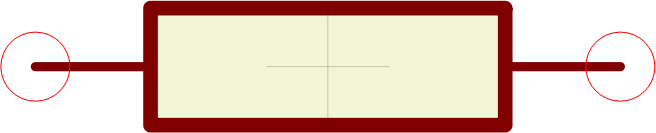
\includegraphics[height=4mm]{images/R-EU_symbol.png}
          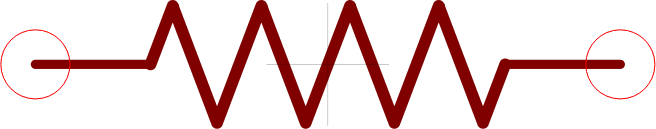
\includegraphics[height=4mm]{images/R-US_symbol.png}
  \end{itemize}

  \pause

  \textbf{Result}
  \begin{itemize}
    \item Duplicate components (same functionality, different symbol)
  \end{itemize}
\end{frame}

\begin{frame}[fragile]{\secname}
  \vspace*{-2\baselineskip}\leavevmode % reduce space
  \begin{center}
    \begin{tikzpicture}
    \matrix (m) [row sep={7mm,between origins}, column sep={.26\textwidth,between origins}] {
      \onslide<1->{\node (tcmp) [anchor=center] {\textbf{Device}};} &
      \onslide<1->{\node (tcmp) [anchor=center] {\textbf{Component}};} &
      \onslide<6->{\node (tvar) [anchor=center] {\textbf{Variant}};} &
      \onslide<1->{\node (tsym) [anchor=center] {\textbf{Symbol}};} \\

      % rows 1-3
      \node (dev11) [lpbox, text width=15mm, anchor=center] {
        \textbf{R-0603}
      }; & & & \\
      \node (dev12) [lpbox, text width=15mm, anchor=center] {
        \textbf{R-0805}
      }; &
      \node (cmp1) [lpbox, text width=15mm, anchor=center] {
        \textbf{\only<1-2,6->{R}\only<3-5>{R-EU}}
      }; &
      \onslide<6->{\node (var1) [lpbox, text width=15mm, anchor=center] {
        \textbf{EU}
      };} &
      \node (sym1) [anchor=center] {
        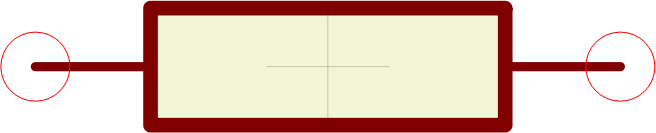
\includegraphics[height=5mm]{images/R-EU_symbol.png}
      }; \\
      \node (dev13) [lpbox, text width=15mm, anchor=center] {
        \textbf{R-1206}
      }; & & & \\

      % rows 4-6
      \onslide<4-5>{\node (dev21) [lpbox, text width=15mm, anchor=center] {
        \textbf{R-0603}
      };} & & & \\
      \onslide<4-5>{\node (dev22) [lpbox, text width=15mm, anchor=center] {
        \textbf{R-0805}
      };} &
      \onslide<3-5>{\node (cmp2) [lpbox, text width=15mm, anchor=center] {
        \textbf{R-US}
      };} &
      \onslide<6->{\node (var2) [lpbox, text width=15mm, anchor=center] {
        \textbf{US}
      };} &
      \onslide<2->{\node (sym2) [anchor=center] {
        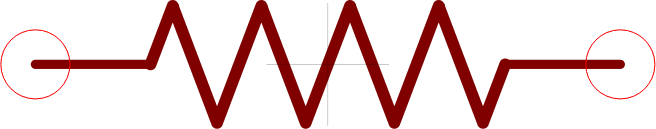
\includegraphics[height=5mm]{images/R-US_symbol.png}
      };} \\
      \onslide<4-5>{\node (dev23) [lpbox, text width=15mm, anchor=center] {
        \textbf{R-1206}
      };} & & & \\

      % rows 7-9
      \onslide<5-5>{\node (dev31) [lpbox, text width=15mm, anchor=center] {
        \textbf{R-0603}
      };} & & & \\
      \onslide<5-5>{\node (dev32) [lpbox, text width=15mm, anchor=center] {
        \textbf{R-0805}
      };} &
      \onslide<5-5>{\node (cmp3) [lpbox, text width=15mm, anchor=center] {
        \textbf{R-small}
      };} &
      \onslide<6->{\node (var3) [lpbox, text width=15mm, anchor=center] {
        \textbf{small}
      };} &
      \onslide<5->{\node (sym3) [anchor=center] {
        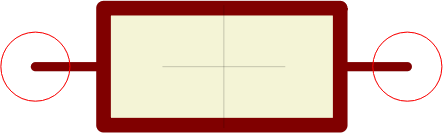
\includegraphics[height=5mm]{images/R-small_symbol.png}
      };} \\
      \onslide<5-5>{\node (dev33) [lpbox, text width=15mm, anchor=center] {
        \textbf{R-1206}
      };} & & & \\
    };

    % box
    \begin{pgfonlayer}{background}
    \onslide<6->{
      \node[fill=yellow!60, fit=(tvar)(var3), inner sep=3mm, rounded corners] {};
    }
    \end{pgfonlayer}

    % lines
    \begin{pgfonlayer}{background}
      % device -> component
      \draw<1->[lpline, draw=red, ultra thick] (dev11.east) -- (cmp1.west);
      \draw<1->[lpline, draw=red, ultra thick] (dev12.east) -- (cmp1.west);
      \draw<1->[lpline, draw=red, ultra thick] (dev13.east) -- (cmp1.west);
      \draw<4-5>[lpline, draw=red, ultra thick] (dev21.east) -- (cmp2.west);
      \draw<4-5>[lpline, draw=red, ultra thick] (dev22.east) -- (cmp2.west);
      \draw<4-5>[lpline, draw=red, ultra thick] (dev23.east) -- (cmp2.west);
      \draw<5-5>[lpline, draw=red, ultra thick] (dev31.east) -- (cmp3.west);
      \draw<5-5>[lpline, draw=red, ultra thick] (dev32.east) -- (cmp3.west);
      \draw<5-5>[lpline, draw=red, ultra thick] (dev33.east) -- (cmp3.west);
  
      % component -> symbol
      \draw<1-5>[lpline, draw=red, ultra thick] (cmp1.east) -- (sym1.west);
      \draw<3-5>[lpline, draw=red, ultra thick] (cmp2.east) -- (sym2.west);
      \draw<5-5>[lpline, draw=red, ultra thick] (cmp3.east) -- (sym3.west);
  
      % component -> variant
      \draw<6->[lpline, draw=red, ultra thick] (cmp1.east) -- (var1.west);
      \draw<6->[lpline, draw=red, ultra thick] (cmp1.east) -- (var2.west);
      \draw<6->[lpline, draw=red, ultra thick] (cmp1.east) -- (var3.west);
  
      % variant -> symbol
      \draw<6->[lpline, draw=red, ultra thick] (var1.east) -- (sym1.west);
      \draw<6->[lpline, draw=red, ultra thick] (var2.east) -- (sym2.west);
      \draw<6->[lpline, draw=red, ultra thick] (var3.east) -- (sym3.west);
    \end{pgfonlayer}
    \end{tikzpicture}
  \end{center}
\end{frame}

\section{Footprint Variants}

\begin{frame}{\secname}
  \textbf{Problem}
  \begin{itemize}
    \item Libraries do not provide an abstraction layer for \textbf{packages}\\
  \end{itemize}

  \begin{center}
    \Huge\textbf{
      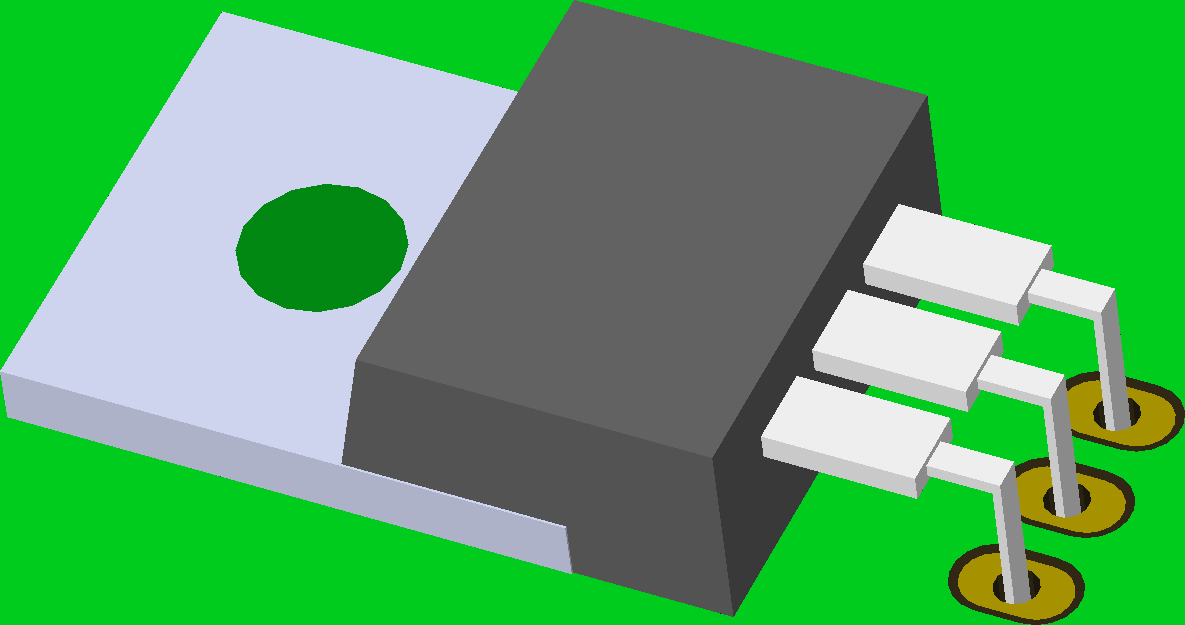
\includegraphics[height=15mm,align=c]{images/TO220_package_normal.png} =
      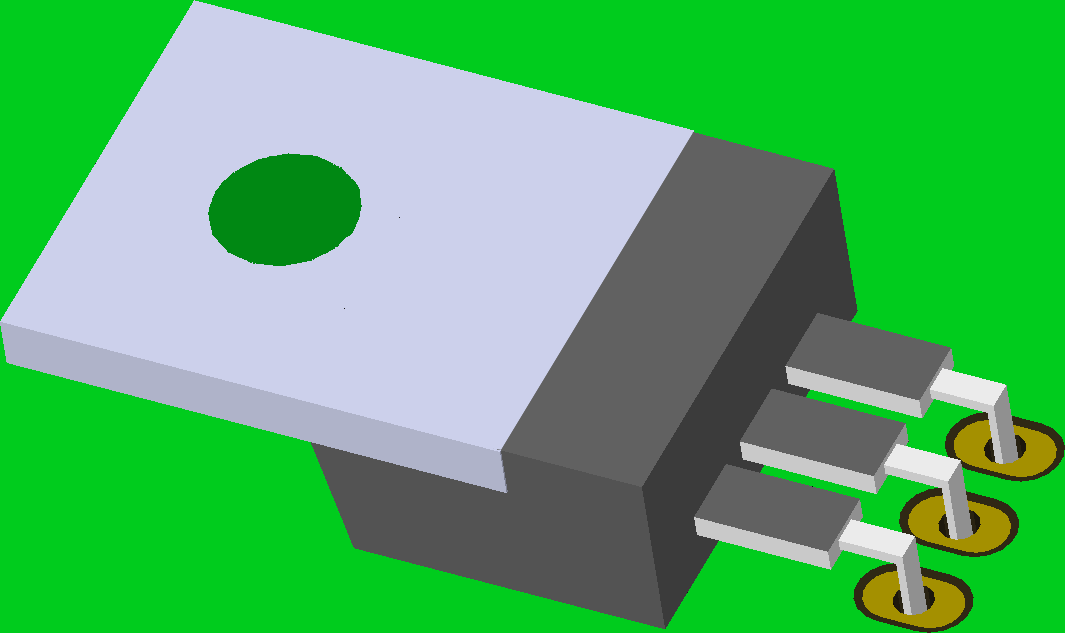
\includegraphics[height=15mm,align=c]{images/TO220_package_reverse.png} =
      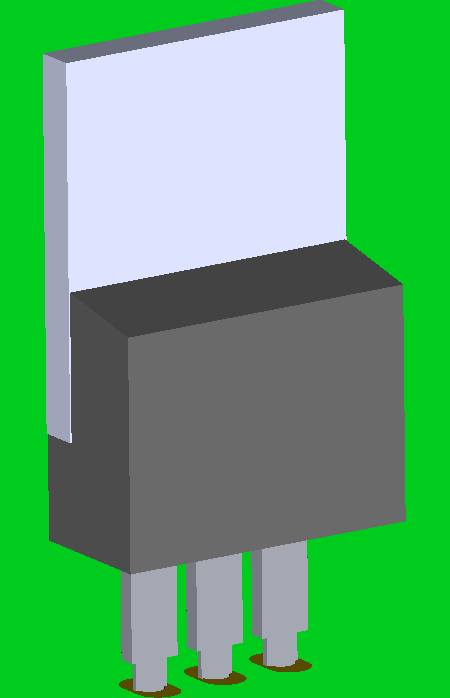
\includegraphics[height=25mm,align=c]{images/TO220_package_vertical.png}
    }
  \end{center}

  \pause

  \textbf{Result}
  \begin{itemize}
    \item Devices need to know every footprint variant of their package
  \end{itemize}
\end{frame}

\begin{frame}[fragile]{\secname}
  \vspace*{-2\baselineskip}\leavevmode % reduce space
  \begin{center}
    \begin{tikzpicture}
      \matrix (m) [row sep={1.7cm,between origins}, column sep={.27\textwidth,between origins}] {
        \node (dev1) [lpbox, text width=2cm, anchor=center] {
          \textbf{LM7805} \\ (Vreg)
        }; & &
        \node (fpt1) [anchor=center] {
          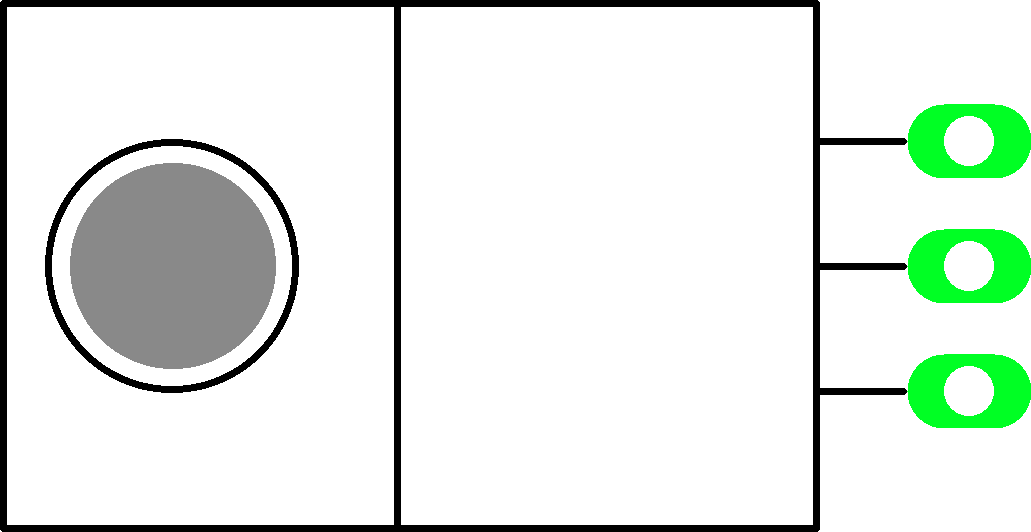
\includegraphics[height=1.2cm]{images/TO220_footprint_normal.png}
        }; &
        \node (pkg1) [anchor=center] {
         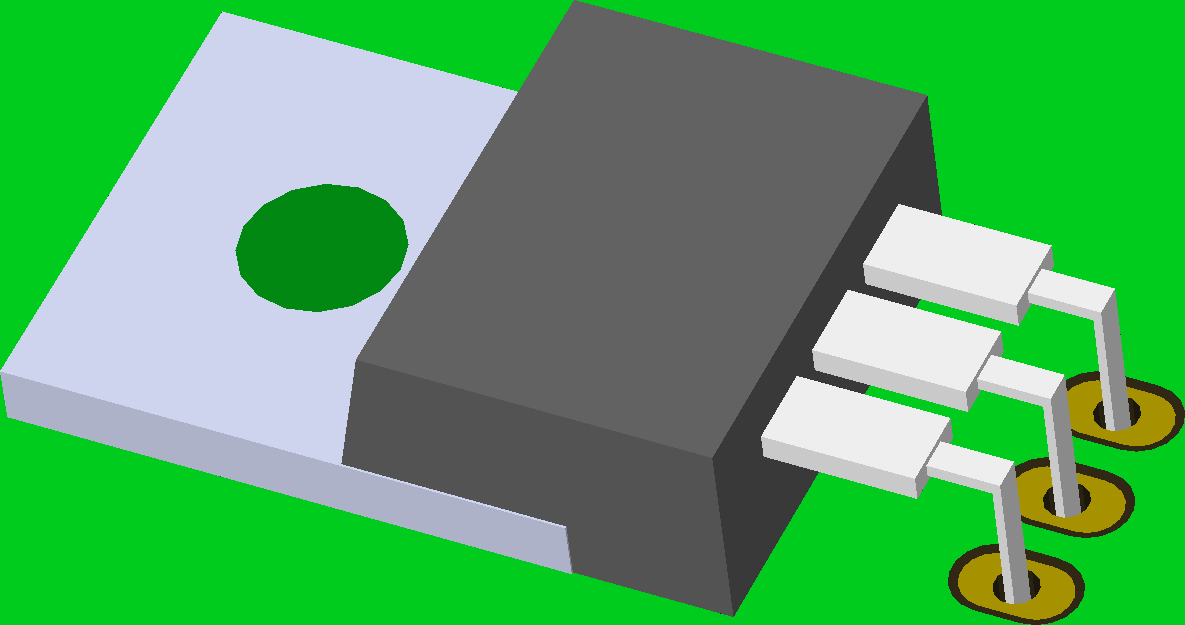
\includegraphics[height=1.2cm]{images/TO220_package_normal.png}
        }; \\

        \onslide<2->{\node (dev2) [lpbox, text width=2cm, anchor=center] {
          \textbf{IRLB8748} \\ (Mosfet)
        };} & &
        \onslide<3->{\node (fpt2) [anchor=center] {
          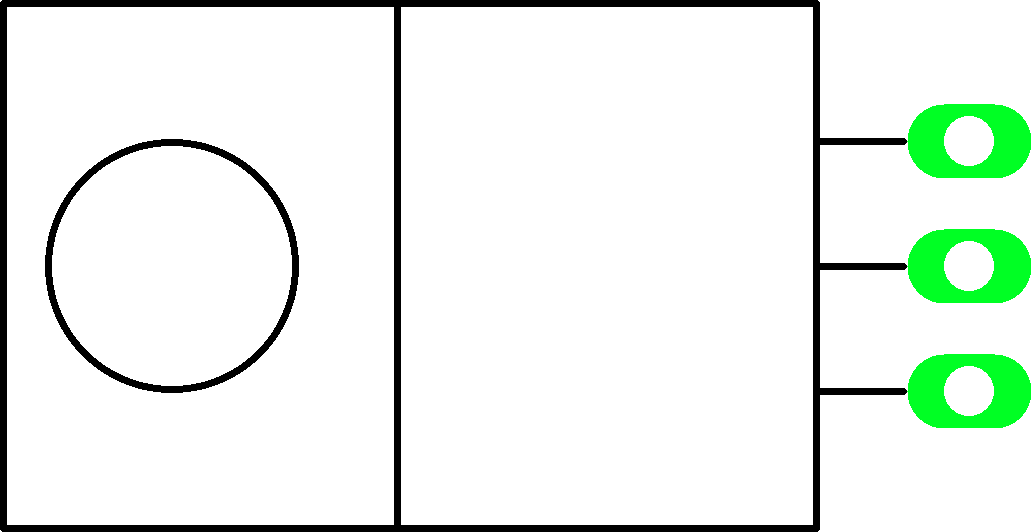
\includegraphics[height=1.2cm]{images/TO220_footprint_nohole.png}
        };} & \\

        \onslide<5->{\node (dev3) [lpbox, text width=2cm, anchor=center] {
          \textbf{MBR40250} \\ (Diode)
        };} & &
        \onslide<7->{\node (fpt3) [anchor=center] {
          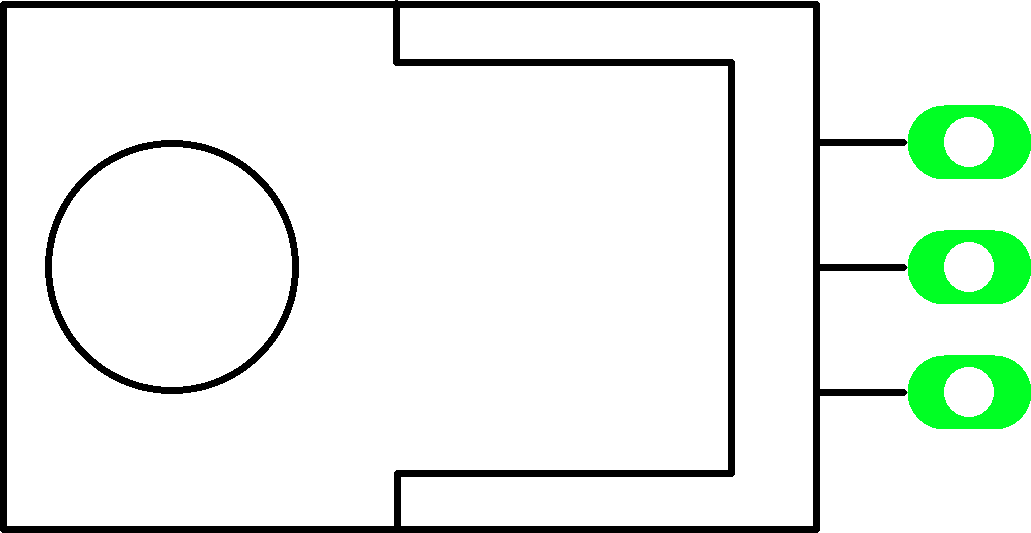
\includegraphics[height=1.2cm]{images/TO220_footprint_reverse.png}
        };} &
        \onslide<7->{\node (pkg3) [anchor=center] {
          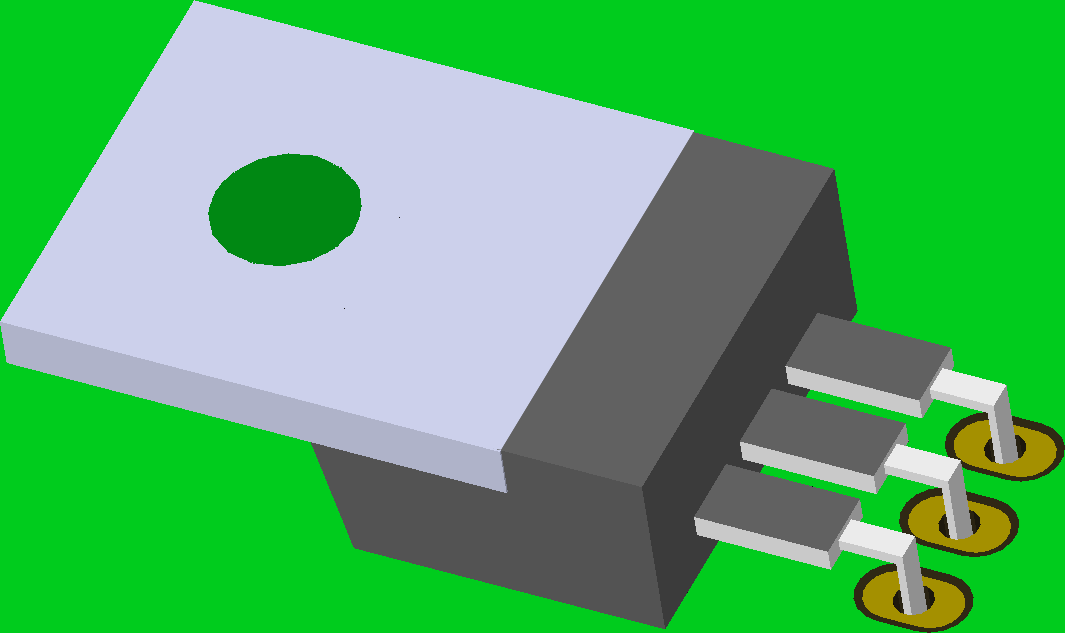
\includegraphics[height=1.2cm]{images/TO220_package_reverse.png}
        };} \\

        \onslide<6->{\node (dev4) [lpbox, text width=2cm, anchor=center] {
          \textbf{DS1821} \\ (Tsensor)
        };} & &
        \onslide<8->{\node (fpt4) [anchor=center] {
          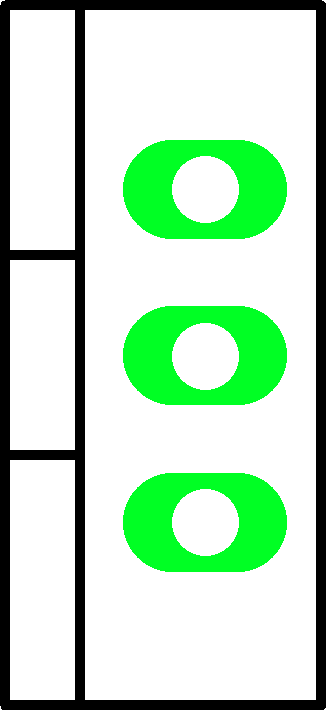
\includegraphics[height=1.2cm]{images/TO220_footprint_vertical.png}
        };} &
        \onslide<8->{\node (pkg4) [anchor=center] {
          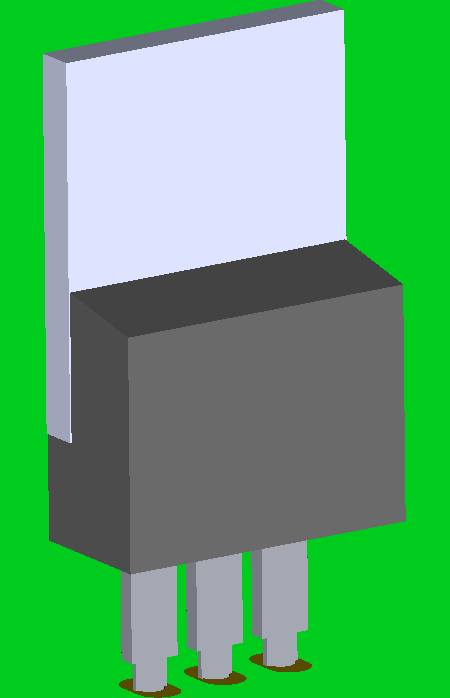
\includegraphics[height=1.2cm]{images/TO220_package_vertical.png}
        };} \\
      };

      \node (tdev) [above=12mm of dev1.center, anchor=center] {\textbf{Device}};
      \node (tfpt) [above=12mm of fpt1.center, anchor=center] {\textbf{Footprint}};
      \node (tmod) [above=12mm of pkg1.center, anchor=center] {\textbf{3D Model}};

      % package
      \onslide<9->{
        \node (tpkg) [anchor=center] at ($(tdev)!0.5!(tfpt)$) {
          \textbf{Package}
        };
        \node (pkg) [lpbox, anchor=center, rectangle split, rectangle split parts=4]
        at ($(dev2)!0.5!(fpt3)$) {
          \textbf{TO-220-3}
          \nodepart{two}   Pad \textbf{1}
          \nodepart{three} Pad \textbf{2}
          \nodepart{four}  Pad \textbf{3}
        };
      }
      \begin{pgfonlayer}{background}
        \coordinate (pkgbot) at ($(dev4.south)!0.5!(fpt4.south)$);
        \onslide<9->{
          \node[fill=yellow!60, fit=(tpkg)(pkg)(pkgbot), inner xsep=5mm, rounded corners] {};
        }
      \end{pgfonlayer}

      \begin{pgfonlayer}{background}
        % footprint -> 3d model
        \draw<1->[lpline, draw=red, ultra thick] (fpt1.east) -- (pkg1.west);
        \draw<3->[lpline, draw=red, ultra thick] (fpt2.east) -- (pkg1.west);
        \draw<7->[lpline, draw=red, ultra thick] (fpt3.east) -- (pkg3.west);
        \draw<8->[lpline, draw=red, ultra thick] (fpt4.east) -- (pkg4.west);

        % device -> footprint
        \draw<1-8>[lpline, draw=red, ultra thick] (dev1.east) -- (fpt1.west);
        \draw<2-8>[lpline, draw=red, ultra thick] (dev2.east) -- (fpt1.west);
        \draw<5-8>[lpline, draw=red, ultra thick] (dev3.east) -- (fpt1.west);
        \draw<6-8>[lpline, draw=red, ultra thick] (dev4.east) -- (fpt1.west);
        \draw<4-8>[lpline, draw=red, ultra thick] (dev1.east) -- (fpt2.west);
        \draw<4-8>[lpline, draw=red, ultra thick] (dev2.east) -- (fpt2.west);
        \draw<5-8>[lpline, draw=red, ultra thick] (dev3.east) -- (fpt2.west);
        \draw<6-8>[lpline, draw=red, ultra thick] (dev4.east) -- (fpt2.west);
        \draw<7-8>[lpline, draw=red, ultra thick] (dev1.east) -- (fpt3.west);
        \draw<7-8>[lpline, draw=red, ultra thick] (dev2.east) -- (fpt3.west);
        \draw<7-8>[lpline, draw=red, ultra thick] (dev3.east) -- (fpt3.west);
        \draw<7-8>[lpline, draw=red, ultra thick] (dev4.east) -- (fpt3.west);
        \draw<8-8>[lpline, draw=red, ultra thick] (dev1.east) -- (fpt4.west);
        \draw<8-8>[lpline, draw=red, ultra thick] (dev2.east) -- (fpt4.west);
        \draw<8-8>[lpline, draw=red, ultra thick] (dev3.east) -- (fpt4.west);
        \draw<8-8>[lpline, draw=red, ultra thick] (dev4.east) -- (fpt4.west);

        % device -> package
        \draw<9->[lpline, draw=red, ultra thick] (dev1.east) -- (pkg.west);
        \draw<9->[lpline, draw=red, ultra thick] (dev2.east) -- (pkg.west);
        \draw<9->[lpline, draw=red, ultra thick] (dev3.east) -- (pkg.west);
        \draw<9->[lpline, draw=red, ultra thick] (dev4.east) -- (pkg.west);

        % package -> footprint
        \draw<9->[lpline, draw=red, ultra thick] (pkg.east) -- (fpt1.west);
        \draw<9->[lpline, draw=red, ultra thick] (pkg.east) -- (fpt2.west);
        \draw<9->[lpline, draw=red, ultra thick] (pkg.east) -- (fpt3.west);
        \draw<9->[lpline, draw=red, ultra thick] (pkg.east) -- (fpt4.west);
      \end{pgfonlayer}
    \end{tikzpicture}
  \end{center}
\end{frame}

\section{Contributing}

\begin{frame}{\secname}
  \begin{centering}
    \bigskip \bigskip
    \textbf{\Huge Contributors welcome!}\\
    \bigskip \bigskip
    {\footnotesize \url{https://github.com/LibrePCB/LibrePCB/blob/master/CONTRIBUTING.md}}\\
    {\footnotesize IRC: \texttt{\#librepcb} on Freenode}\\
  \end{centering}
  \textbf{\Large
    \begin{itemize}
      \centering
      \item Participate in issues
      \item Open pull requests
      \item Improve documentation
      \item Donate (Patreon, GitHub Sponsors, \dots)
    \end{itemize}
  }
\end{frame}


% ----------------------------------------------------------------- %

{
\setbeamertemplate{footline}{}
\begin{frame}[standout]
	\begin{centering}
	{\Huge Thank you!}\\
	{\normalsize \url{http://librepcb.org}}\\
	\end{centering}
\end{frame}
}

% ----------------------------------------------------------------- %

\end{document}
